\chapter{Metode}

\section{Razvojno okolje}
Ves razvoj je potekal v programskem okolju MATLAB. Ta poleg samega programskega jezika vsebuje velik nabor že implementiranh funkcij, napredne aplikacije za strojno učenje in knjžnice ki omogočajo povezave z laboratorjskimi napravami. V njem sta ustvarjeni funkciji za računanje matric Grangerjevega indexa vzročnosti
in matric Kompleksnega Pearsonov korelacijskega koeficienta. V njem so ustvarjene nevronske mreže in uporabljeno je za ostale klasifikatorje. Prav tako smo v njem napisali funkcijo za zajemanje podatkov iz naprave Cognionics Quick-20, funkcijo ki v realnem času razpoznava gibanji.
    
\subsection{EEGLAB}
EEGLAB je interaktivna matlab orodjarna, za procesiranje in obdelavo elektrofizioloških podatkov. Omogoča rereferenciranje EEG signalov, izbiro določenih elektrod, deljenje podatkov na epohe glede na dogodke in filtriranje frekvenc. Omogoča interakcijo preko uporabniškega vmesnika. Vse akcije v vmesniku se prevedejo v ukaze ki jih lahko uporabimo v svoji kodi. Pri izdelavi naloge smo največ uporabljali funkcije branja .edf datotek, filtriranja frekvenc signalov in deljanja posnetkov na manjše dele.\cite{noauthor_eeglab_nodate}

\subsection{Lab streaming layer}
Lab streaming layer je odprtokodna vmesna programska oprema ki omogoča pošiljanje, prejemanje, sinhronizacijo in snemanje tokov podatkov. Omogoča enostavno povezovanje EEG naprave z programsko opremo MATLAB. Knjižnjico je potrebno prenesti in nato zgraditi na svojem računalniku.  \cite{noauthor_lsl-website_nodate}

\section{EEG Motor Movement/Imagery Dataset}
EEG Motor Movement/Imagery Dataset je prosto dostopna zbirka več kot 1500 eno in dve minutnih posnetkov 109 prostovoljcev ki opravljajo različne naloge. Za nas relevantni so posnetki serij 3, 5 in 7 v katerih prostovoljci stiskajo in sproščajo levo ali desno pest. Posnetki so shranjeni v formatu EDF+ ki vsebuje posnetke EEG in oznake dogodkov. Snemanje je bilo opravljeno s frekvenco 160Hz in 64 elektrodnim sistemom EEG.\cite{schalk_eeg_2009,schalk_bci2000_2004}

\section{Metode povezljivosti}
\subsection{Grangerjev index vzročnosti}
Grangerjev index vzročnosti je statistična metoda za preverjanje ali ena časovna vrsta nosi informacije o drugi. Metoda je bila razvita v šestdesedih letih devetnajstega stoletja za uporabo ekonomiji.

Za dve časovni vrsti $X_1$ in $X_2$, in $p$ kot število prejšnjih vrednosti ki jih upoštevamo pri računanju, lahko izračunamo $E_1$ in $E_1$ ki so napake pri predvidevanju naslednje vrednosti v vrsti $X_1$. V kolikor je varianca vrednosti $E_2$ manjša kot varianca vrednosti $E_1$ lahko predvidevamo da časovna vrsta $X_2$ nosi informacije o časovni vrsti $X_1$
\begin{align*}
X_1(t) &= \sum_{j=1}^{p} A_{1,j} X_1(t-j) + E_1(t)\\
X_1(t) &= \sum_{j=1}^{p} A_{2,j} X_1(t-j) + \sum_{j=1}^{p} A_{3,j} X_2(t-j) + E_2(t)
\end{align*}


\textcolor{red}{Mogoče razlaga kaj so A-ji. Ali so pravilno zapisani?}

\cite{seth_granger_2007}

\subsection{Kompleksni Pearsonov korelacijski koeficient}
Pearsonov korelacijski koeficient je najpogosteje uporabljen linearni korelacijski koeficient. Zanj smo se odločili saj v članku  \citetitle{sverko_complex_2022} avtorji pokažejo da vsebuje informacije PLI in wPLI ki sta dve najbolj pogosto uporabljeni metodi povezljivosti. Za naš primer lahko uporabimo enačbo s kompleksnimi števili:

\begin{align*}
r(X_1, X_2) &= \frac{\sum\limits_{n=1}^{N} X_{1,n} \cdot \overline{X_{2,n}}}{\sqrt{\sum\limits_{n=1}^{N} |X_{1,n}|^2} \cdot \sqrt{\sum\limits_{n=1}^{N} |X_{2,n}|^2}}.
\end{align*}
\textcolor{red}{Kaj predstavlja pika na koncu enačbe?}


\cite{sverko_complex_2022} 

\section{Klasifikacija}
Na pridobljenih matrikah povezljivosti smo preizkusili več vrst klasifikacije in sicer: odločitvena drevesa, metodo k najbližjih sosedov (k-NN), logistično regresijo, podporne vektorske stroje (SVM) in nevronske mreže.
\subsection{Classification learner}
Classification learner je aplikacija v Matlabu za enostavno klasifikacijo podatkov. Podpira različne metode klasifikacije, navzkrižno validacijo in uporabo različnih podatkov za gradnjo in testiranje modela.
\subsection{Nevronska mreža}
Nevronska mreža je sestavljena iz vhodne plasti za slike dimenzij 19x19x1, polno povezanega sloja s 100 nevroni, Leaky ReLU sloja, dropout sloja z 50\% verjetnostjo opustitve nevronov, polno povezanega sloja z 10 nevroni, GELU sloja, dropout sloja z 50\% verjetnostjo opustitve nevronov, polno povezanega sloja s tremi nevroni in Softmax sloja.
\begin{figure}[h!]
\begin{center}
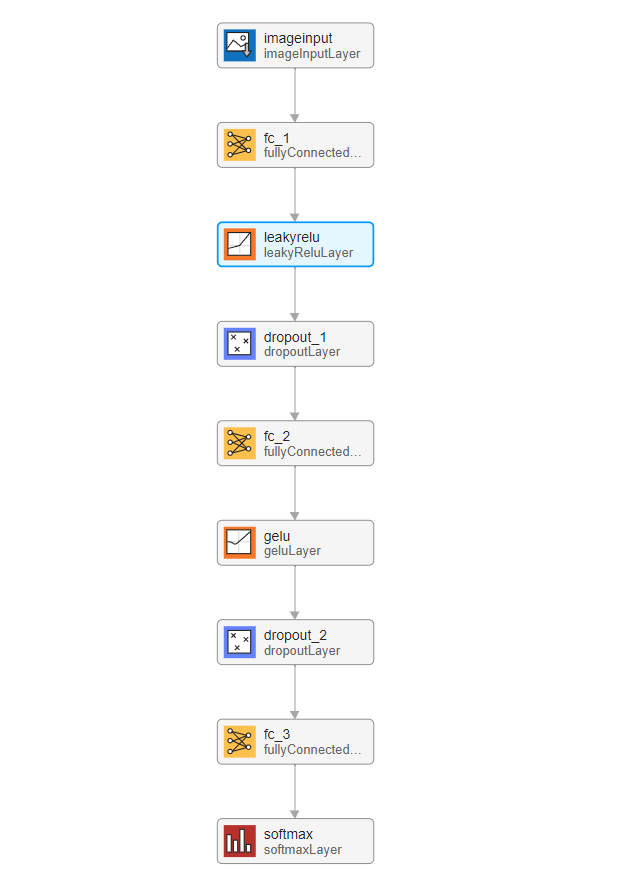
\includegraphics[width=0.5\linewidth]{slike/Neural network.png}
\end{center}
\caption{Nevronska mreža.}
\end{figure}

\section{Filtriranje}
Knjižnica EEGLAB nam omogoča filtriranje signalov naprej in nazaj? kar v našem primeru ni primerno saj podatke prejemamo sekvenčno. Zato smo podatke filtrirali s pomočjo filtra z stanji ki nam omogoča filtriranje sekvenčnih podatkov. Ker pa filtra nista enakovredna, saj prvi ohranja zamike faz drugi pa ne, uporabljena metoda CPCC pa deluje na zamikih faz, smo izvedli dodatno testiranje da smo preverili če pristop deluje enako učinkovito.



